Even though a lot of visualisation tools for different use cases emerged, there is only a small amount of tools trying to animate the transition between two visualisations. This chapter provides three types of exemplarily selected tools:

\newpage
\begin{enumerate}
\item tools that use some kind of animation to create the visualisation,
\item tools that also allow creating maps and
\item tools that try to animate the transition when changing the visual appearance.
\end{enumerate}

In order to evaluate all presented works with the same base, the analysis framework mentioned in Chapter \ref{s:basics} on page \pageref{s:basics} is used.

\subsubsection{Gapminder}
Gapminder\footnote{See \href{https://www.gapminder.org/}{https://www.gapminder.org/}} is very well known in the information visualisation community and the content of the data it uses is entirely explored. It shows wealth and health of countries over time and has more than 500 datasets as a basis. The default visualisation of gapminder is an extended scatter plot where the x-axis shows income per person, the y-axis life expectancy in years, the bubble itself represents the total population of each country by size and the color indicates the region of the country. Furthermore, the scatter plot is expanded with a timeline. The interactive demo of Gapminder also allows users to inspect different indicators of wealth and health.

\begin{figure}[!htb]
\centering
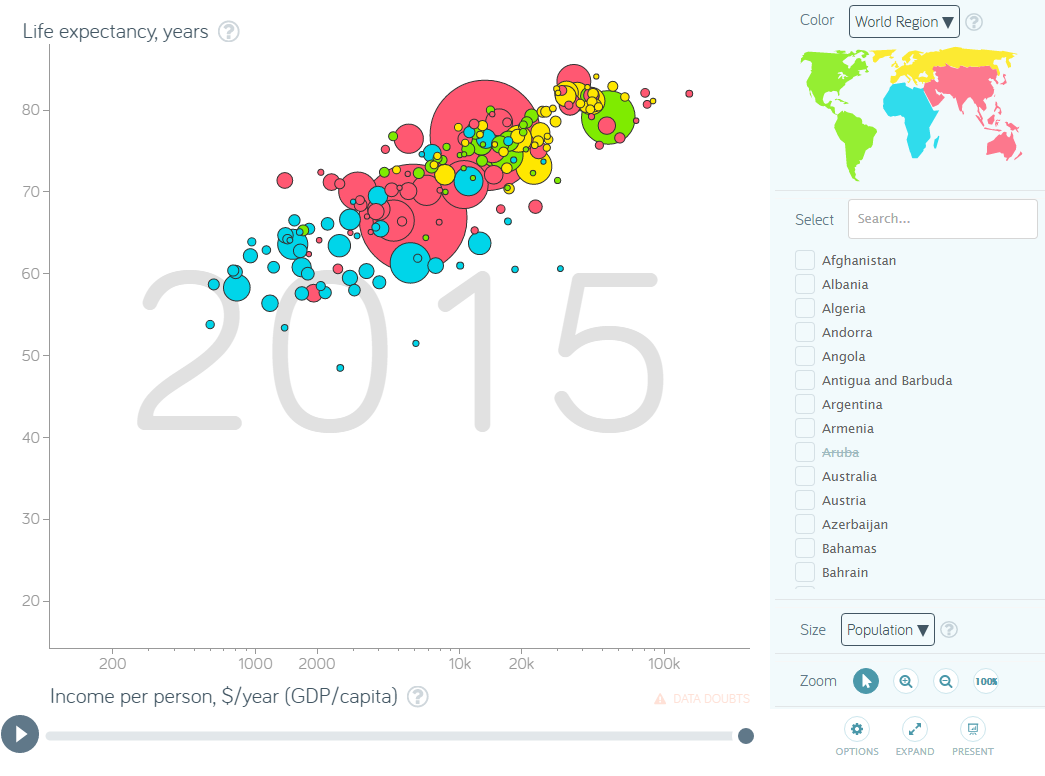
\includegraphics[height=5cm]{images/methods/related/gapminder.png}
\caption[
    Gapminder
]{Gapminder}
\label{fig:gapminder}
\end{figure}

Gapminder is not visualisation tool, but demonstrates a very popular example of animation in visualisations as a practical example. Figure \ref{fig:gapminder} on page \pageref{fig:gapminder} shows the application displaying the data corresponding to the year 1904. Users have some control over the visualisation shown:
\begin{itemize}
\item changing the attributes mapped,
\item controlling the animation by playing and pausing it directly,
\item selecting the countries which are of interest and
\item setting the symbol size.
\end{itemize}

The application made it possible to discover that people live longer in countries with a higher \ac{GDP} per capita. Countries with a low income have really short life expectancy. Furthermore, it is also discovered, that living in middle-income countries, the lifespan is huge, depending on how the income in the country is distributed and used.


\subsubsection[A Unifying Framework for Unit Visualisations]{A Unifying Framework for Animated and Interactive Unit Visualisations}
\citeauthor{Drucker2015} describe a tool which makes use of so called unit visualizations. This type of visualization is best described as using one complete row of a dataset and representing it as a unit. Advantages of using units are described in the following list \iacite{Drucker2015}:
\begin{itemize}
\item \textbf{The forest and the trees:} when using a visualization based on aggregation of data, it is possible to hide outlying data or have outlying data influence the representation \iacite{Drucker2015}. However, unit visualizations maintain a one-to-one correspondence between rows in a dataset with the represenation. While classical bar charts only show one static bar for each aggregated attribute, unit visualizations show the dynamic units building that bar. Therefore, a bar for a bar chart made in a unit visualization is not a single, static shape. It is a dynamically created bar with shapes representing each unit individually and thus showing the trees yielding the forest instead of showing only the forest.

\item \textbf{Semantic constancy:} the connection between a row and a unit is maintained throughout all changes. Thus, changing visual attributes or switching from one visualization to another, does not break that bond.

\item \textbf{Direct interaction:} when using the concept of unit visualizations, it is fairly easy to show additional information of each unit by providing for example tooltips. Even when using multiple views, the concept of linking and brushing (see chapter \ref{s:linking-brushing} on page \pageref{s:linking-brushing} fore more information) can be accomplished by highlighting the selected units in every view. Furthermore, if some kind of aggregated visualization is implemented with this concept, the units can still be highlighted because they are still visible.

\item \textbf{Animation:} because of the semantic constancy, it is possible to animate smoothly between different visualizations. Transitions only update the position of every unit since they are all present.

\end{itemize}

Albeit showing a lot of advantages, the concept of unit visualizations show some weaknesses:

\begin{itemize}
\item Using a lot of units, for example, in a bar can lead to visual clutter compared to a single, static aggregated one.

\item Accessing the information of the aggregation needs more calculation in a unit visualization because each unit already represents its row and still needs to know its particular group for aggregation. First, this group needs to be calculated and second, some attributes e.g. count or sum needs to be shown in the visualization.

\item Scaling is the main weakness of this type of visualizations. Aggregate visualizations can potentially use a much larger dataset, compared to unit visualizations. Scaling does not only include the amount of data used, it also includes the hardware accessible. Displaying thousands of items and animating them requires more operation power than calculating an aggregation and drawing a rectangle on a fixed position.

\end{itemize}

\begin{figure}[!htb]
\centering
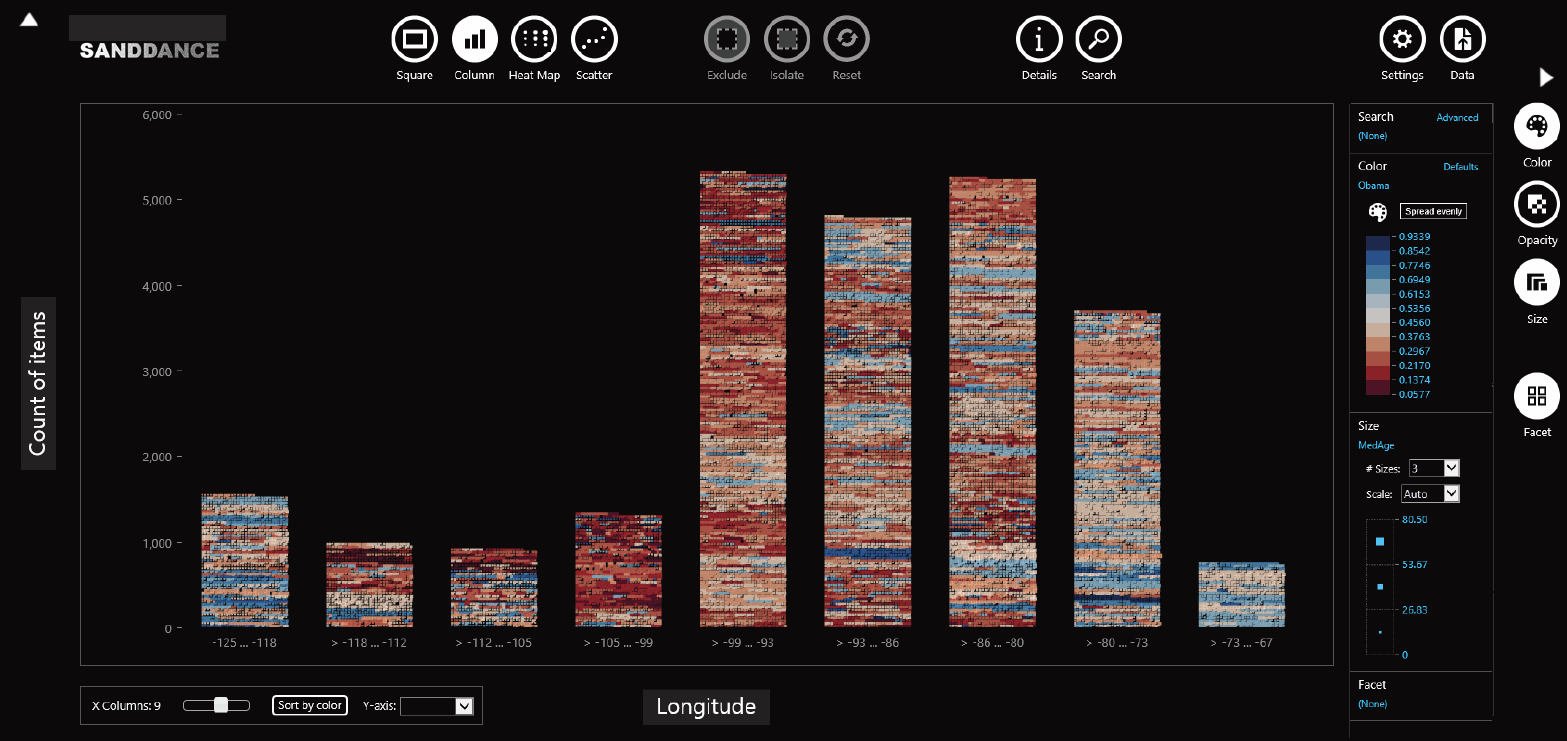
\includegraphics[width=0.8\textwidth,keepaspectratio]{images/methods/related/sanddance.png}
\caption[
    Concept of SandDance \iacite{Drucker2015}.
]{SandDance}
\label{fig:sanddance}
\end{figure}

Figure \ref{fig:sanddance} on page \pageref{fig:sanddance} shows the prototype. It allows to manually change visual channels to the right and change visual appearance e.g. changing the type of visualization at the top left. According to the analysis framework, SandDance uses static tables as input data only. \citeauthor{Drucker2015} states, that the tool was built to explore the benefits of using unit visualizations. Therefore it has no real use case to analyse, because it was used to show a completly different type of visualization without considering user benefit. However, one could say that the tool can be used to consume information and maybe discover new knowledge if using non-preexistent datasets.
SandDance can be still analysed when looking at how they implemented the visualization idiom: they freely allow users to encode attributes, even suggesting appropriate values automatically. Manipulation is implemented with a possible change in visual appearance and selection of shown data. The selection can further be filtered in different ways by either isolating or excluding data based on the given criteria.
Based on the three different types of tools already mentioned, SandDance counts as a tool supporting multiple views with different types of visualizations including maps. Furthermore it animates the transition when changing visual appearance in some kind of linear but not understandable way. Creating a new visualization is also animated with the same concept.


\subsubsection{Visual Sedimentation}
\citeauthor{Huron2013} developed a novel design metaphor inspired by the physical process of sedimentation. The design metaphor is called visual sedimentation and describes the process of aggregating falling objects due to gravity over time into static shapes \iacite{Huron2013}. This concept can be applied very well to streamed data. Incoming data items would be represented by falling objects, animated by virtual forces and aggregating over time in static shapes.
The basic concept of visual sedimentation can be described in four steps:

\begin{enumerate}
\item A new data item is processed and "enters" the scene.
\item Virtual forces are applied to the data item and suspension occurs while falling to the ground.
\item Items are accumulated on the ground or on top of previous items.
\item Items are merged into an aggregated shape.
\end{enumerate}

The possible datasets for visual sedimentation are quite obvious: all the examples discussed in the paper are some kind of dynamic, streamed data including a temporal attribute. This fact already answeres the first question of the analysis framework. Nonetheless, the concept and the examples could be extended with using static datasets without any kind of attribute of a temporal nature. Preprocessing and sorting the dataset before dropping items into the scene could yield interesting results. The weakness of using static datasets is that it stops after every item being processed. Aggregating an item into a static shape is based on multiple decisions in visual sedimentation. Thus it yields to non-aggregated data items on top of an aggregated shape when the dataset is finished. This does not happen when using streamed data.
The reason that visual sedimentation does not allow any kind of interaction leads to the answer of why even use it. It is mainly used to present some kind of data and to enjoy the visualisation itself. It is not possible to get more information on neither a single data item nor an aggregated shape.
The discussed examples are all based on two facts:
\begin{enumerate*}
\item all of them use streamed data including a temporal variable and
\item all data items have the same categorical attribute.
\end{enumerate*}
Thereby, visual sedimentation makes use of visualisations which are able to handle categorical data and use color as the visual encoding channel.

\begin{figure}[!htb]
\centering
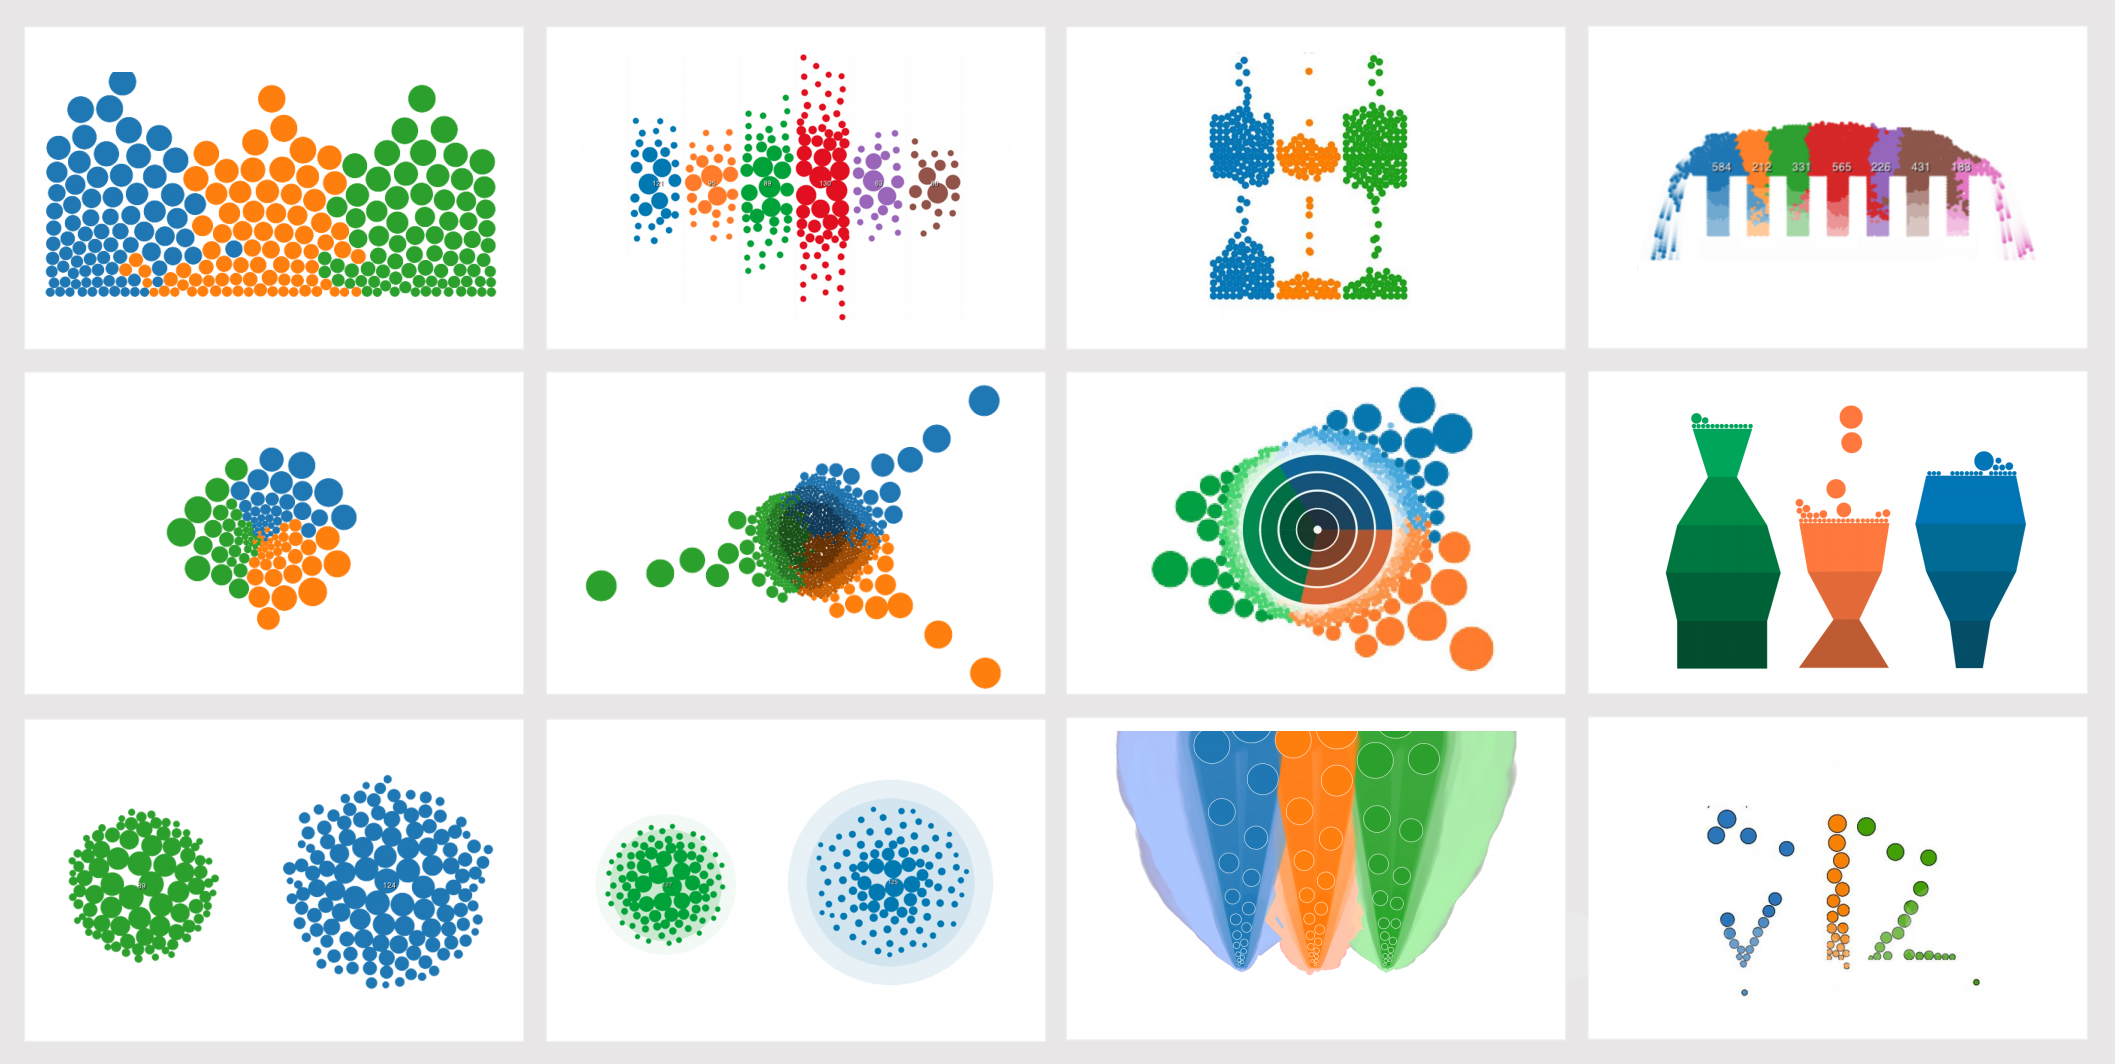
\includegraphics[height=5cm]{images/methods/related/visual-sedimentation}
\caption[
    Charts created by visual sedimentation \iacite{Huron2013}.
]{Charts created by visual sedimentation}
\label{fig:visual-sedimentation}
\end{figure}

Figure \ref{fig:visual-sedimentation} on page \pageref{fig:visual-sedimentation} shows possible charts made by visual sedimentation.

\subsubsection{Animated Transitions in Statistical Data Graphics}
\citeauthor{Heer2007} describe a tool called DynaVis which makes use of animated transitions between different visualisations. Users often switch the type of a visualisation in order to answer different questions concerning underlying data. However, doing this transition in a static way leads to information loss of the former visualisation. Thus, animating the transition of the current visualisation to the upcoming one could result in better comprehensibility of the upcoming visualisation. The cruical point of an animated transition is to keep the users oriented during the transition. The best case of an animated transition would be that users are able to accurately identify elments across disparate visualisations and understand the connections between them.

\citeauthor{Heer2007} investigate the design of animated transitions between statistical data graphics. Furthermore, they propose design guidelines for animated transitions which are discussed below. The primary contribution of \citeauthor{Heer2007} is two conducted user studies to assess the efficiency of animated transitions \iacite{Heer2007}.

The following design principles can be categorised into two sections: congruence and apprehension. All principles are taken from \citeauthor{Heer2007} and each one of them is listed and shortly discussed below \iacite{Heer2007}.

\begin{itemize}
\item \textbf{Congruence}
\begin{description}
\item[Maintain valid data graphics during transitions.] This design principle suggests that the interpolation states between two visualisations remain valid data graphics in order to minimise unwarranted attributions to the data.
\item[Use consistent semantic-syntactic mappings.] This principle recommends to use similar transitions for a single purpose throughout the visualisation tool. This ensures consistency across all available visualisation types.
\item[Respect semantic correspondence.] If a mark represents specific data points, it should not be reused to depict different data points in a transition.
\item[Avoid ambiguity] because it increases the risk of misinterpretation.
\end{description}

\item \textbf{Apprehension}
\begin{description}
\item[Group similar transitions.] Objects undergoing similar visual changes at the same time support comprehensibility of users due do perceptual grouping.
\item[Minimise occlusion.] Tracking occluding objects during a transitoin is unreasonable and also harming perception.
\item[Maximising predictability] of a transition reduces cognitive load and improves tracking abilities.
\item[Use simple transitions] because complex transitions with unpredictable movement would increase cognitive load.
\item[Use staging for complex transitions.] This allows for breaking down complex transitions into simple ones. Staging multiple simple transitions decreases cognitive load increases observability.
\item[Make transitions as long as needed, but no longer.] Slow transitions can result in longer task times and diminished engagement. However, they should still be long enough for accurate change tracking.
\end{description}

\end{itemize}

DynaVis is shown in Figure \ref{fig:dynavis} on page \pageref{fig:dynavis}. It features two different types of animated transitions from a scatter plot to a bar chart. The top path directly interpolates between the starting and ending visualisation, whereas the bottom path makes use of staging. The points in the scatter plot move to their corresponding x-coordinate and the axis is updated. Afterwards, the points are morphed into bars resulting in the desired visualisation.

\begin{figure}[!htb]
\centering
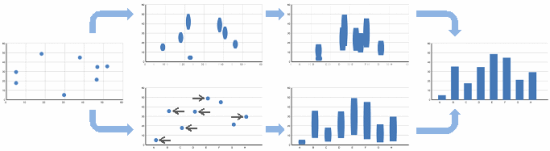
\includegraphics[width=0.8\textwidth, keepaspectratio]{images/methods/related/dynavis.png}
\caption[
    DynaVis \iacite{Heer2007}.
]{DynaVis}
\label{fig:dynavis}
\end{figure}

The herein before mentioned user studies concerning the effectiveness of DynaVis showed, that animated transitions support the user's perception and increases the readability of the visualisation. Furthermore, the studies showed that staged animations are preferred compared to direct interpolations.

In summary, using staged animations with considering the mentioned design principles could also work for geo-spatial visualisations. Thus, it could support the understandability and readability of different types of geo-spatial visualisations.

\subsubsection{Visual Analysis of Anomalous Information Spreading on Social Media}
\citeauthor{Zhao2014} present an interactive visual analysis system designed for revealing and analyzing anomalies spreading in social media. The main challenge of such a system is to distill valuable information from streamed social media data, due to the heterogeneous and dynamic crowd behaviours \iacite{Zhao2014}. The challenge is not further described in this thesis because it is irrelevant as related work. However, some parts of the visual analysis system are very interesting and worth a rough analysis.

Figure \ref{fig:fluxflow} on page \pageref{fig:fluxflow} shows FluxFlow. It is based on multiple views combined with linking and brushing. As one can see, it deconstructs heterogeneous social media data and builds some kind of tree. The tree can be navigated and single nodes can be highlighted with hovering. Clicking on a single node creates a new view showing all its subnodes as circles on a timeline. The radius of the circle depends on an attribute of the data item. The creation of the timeline is linear animated. Each click on a node appends a new timeline in given view.

\begin{figure}[!htb]
\centering
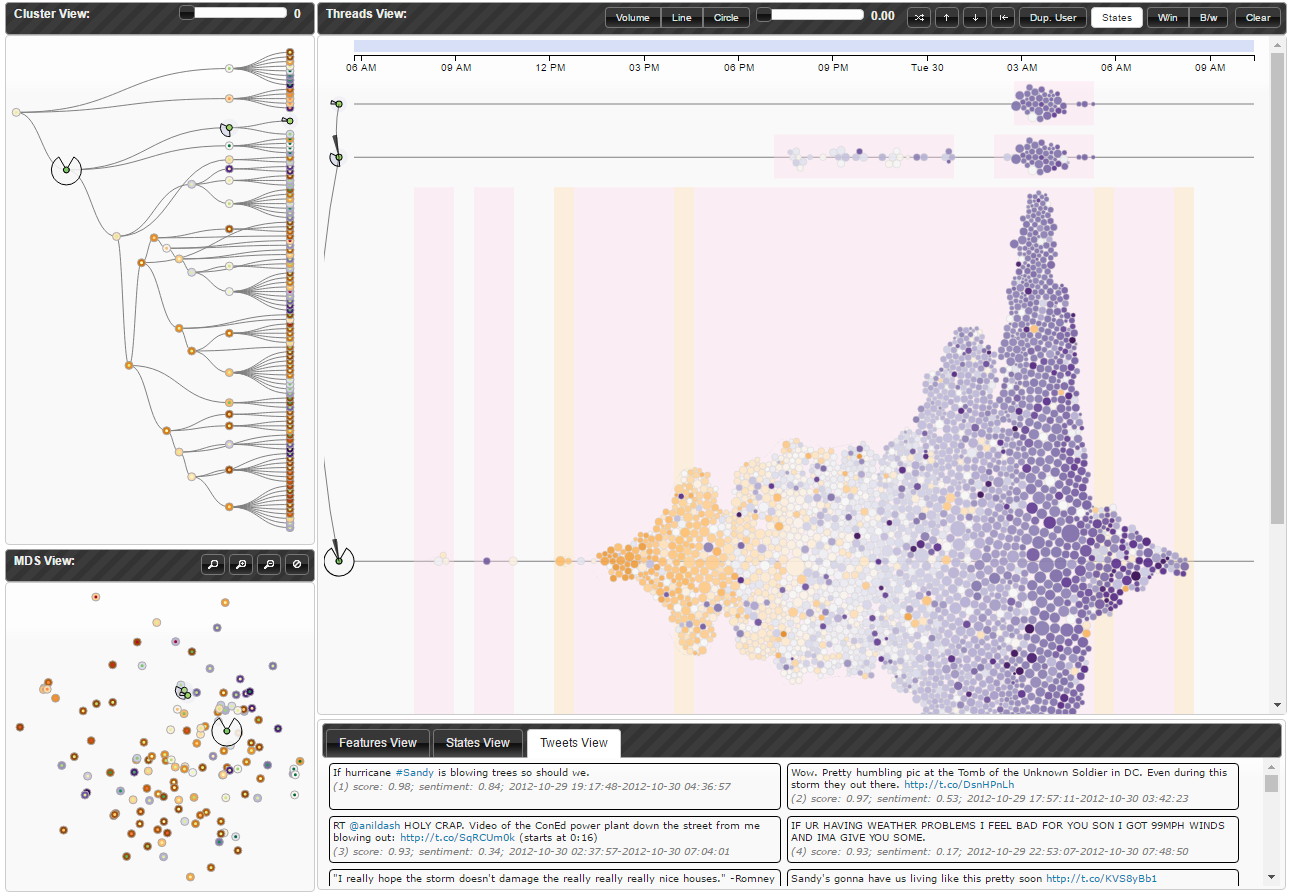
\includegraphics[height=5cm]{images/methods/related/fluxflow.png}
\caption[
    Fluxflow: a visual analysis system \iacite{Zhao2014}.
]{Fluxflow: a visual analysis system}
\label{fig:fluxflow}
\end{figure}

The use case of such a system is very well described in the paper, therefore making it easy to analyze possible datasets. Even though the main challenge of the system is to analyze streamed data, the visualisation itself is only based on static datasets. It is not clear if the system is able to build the tree from a table dataset itself or if the tree must be given.
The objective of FluxFlow is to show anomalies in social media data and discover insights with using the multiple view system combined with multiple visual channels and interaction methods. Manipulating the visualisation is possible through interaction with the timeline, selecting interesting nodes in the tree or entering specific time slots to view.
